
\documentclass{beamer}
\usetheme{Madrid}
\usepackage{graphicx,harvard}
\usepackage{qtree}
\title{Structure and meaning}
\author{Liam Keeble}
\institute{School of English Literature, Language and Linguistics}
\date{}



\begin{document}


\frame{\titlepage}

\begin{frame}{Introductions}
\begin{itemize}
\item Who am I?
\item What is this module about?
\item How is it going to run?
\end{itemize}
\end{frame}

\begin{frame}{Overview}
\tableofcontents
\end{frame}



\section{The problem of language structure}

\begin{frame}{The problem of language structure}
	\begin{itemize}
	\item How would a Martian figure it out?
	\item 'John did go to the shop'
	\item Auxiliary verbs such as 'did' always come after the first word in a sentence
	\end{itemize}
\end{frame}

\begin{frame}{The problem of language structure}
	\begin{itemize}
	\item But what about...
	\item 'The man with the hat did go to the shop'
	\item We can't have 'The did man with the hat go to the shop'
	\item So how do we solve this problem?
	\end{itemize}

\end{frame}

\begin{frame}{How do we solve this problem?}
	\begin{itemize}
	\item Analytic philosophy
	\item Breaking language down into its smallest units of meaning...
	\item And building it back up again
	\end{itemize}

\end{frame}

\begin{frame}{Intuition}
	\begin{itemize}
	\item Our intuitions are useful
	\item We know what sounds right, but we need to figure out why
	\item And when we say 'right' we mean what sounds right, not what we are told is right by dusty old grammar books...
	\end{itemize}


\end{frame}

\section{Foundations}

\begin{frame}{Where is language?}
	\begin{itemize}
		\item I-language: the capabilities human beings have to construct linguistic structures in the brain (competence)
	\item E-language: the externalisation of language (e.g. things that speakers say, also know as utterances/performance)
	\end{itemize}

\end{frame}


\begin{frame}{What is language?}
	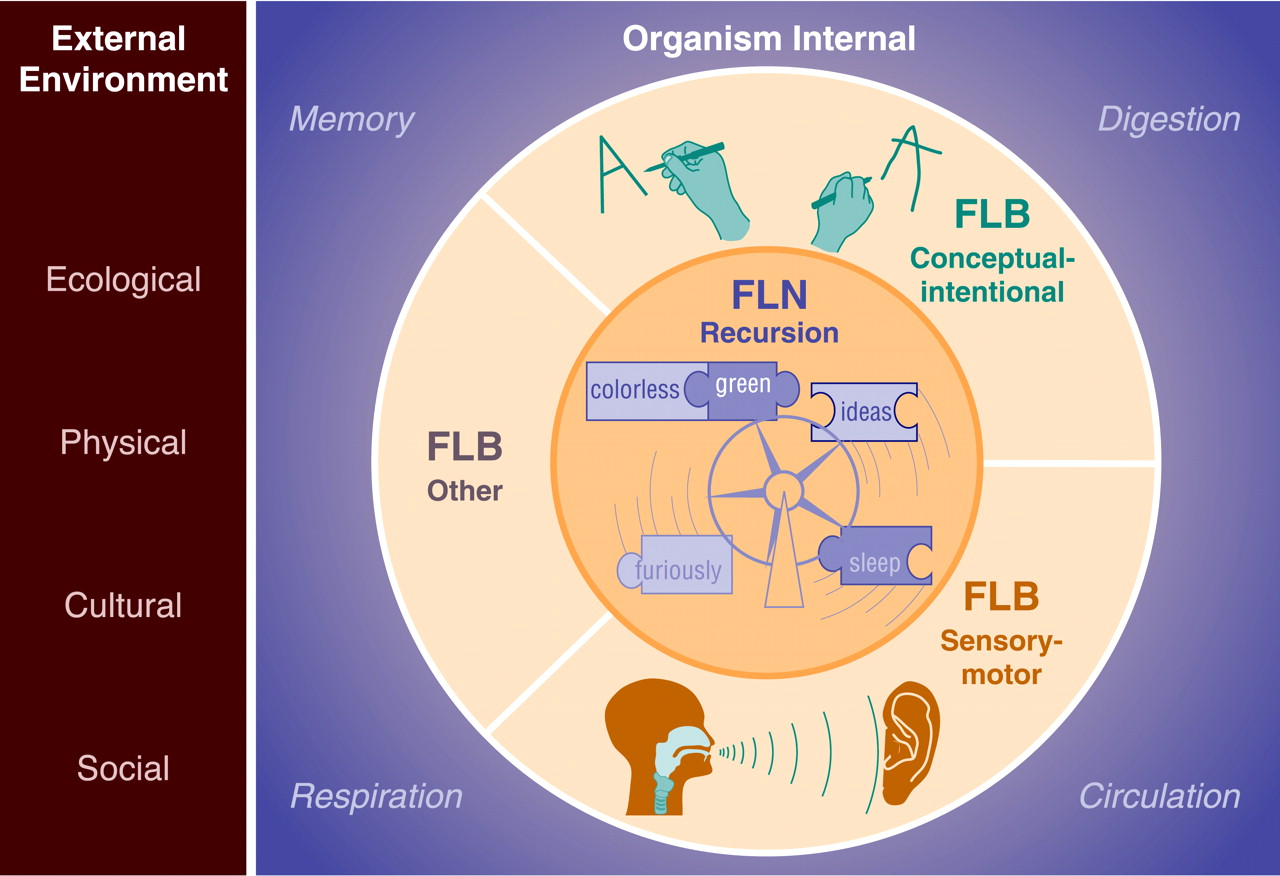
\includegraphics[scale=0.25]{FLN.jpg}
	\nocite{hauser2002faculty}
\end{frame}



\section{Structure in words}

\begin{frame}{Morphology and meaning}
	\Tree [.V un- [.V lock ] ]
	\vspace{2cm}

	\Tree [.A [.V un- [.V lock ] ] -able ]

\end{frame}

\begin{frame}{Morphology and meaning}
	\Tree [.N [.A [.V un- [.V lock  ] ] -able ] -ism ]

	\Tree [.N [.A [.V un- [.V lock ] ] -able ] -ology ]
\end{frame}

\section{Structure in sentences}

\begin{frame}{Syntax and meaning}

\end{frame}



\begin{frame}{References}
\bibliographystyle{agsm}
\bibliography{references.bib}
\end{frame}


\end{document}















